%%%%%%%%%%%%%%%%%%%%%%%%%%%%%%%%%%%%%%%%%%%%%%%%%%%%%%%%%%%%%%%%%%%%%%%%%%%%%%%%%%%%%%%%%%%%%%%%
%
% CSCI 1430 Written Question Template
%
% This is a LaTeX document. LaTeX is a markup language for producing documents.
% Your task is to answer the questions by filling out this document, then to
% compile this into a PDF document.
%
% TO COMPILE:
% > pdflatex thisfile.tex
%
% If you do not have LaTeX and need a LaTeX distribution:
% - Departmental machines have one installed.
% - Personal laptops (all common OS): http://www.latex-project.org/get/
%
% If you need help with LaTeX, come to office hours. Or, there is plenty of help online:
% https://en.wikibooks.org/wiki/LaTeX
%
% Good luck!
% Srinath and the 1430 staff
%
%%%%%%%%%%%%%%%%%%%%%%%%%%%%%%%%%%%%%%%%%%%%%%%%%%%%%%%%%%%%%%%%%%%%%%%%%%%%%%%%%%%%%%%%%%%%%%%%
%
% How to include two graphics on the same line:
%
% \includegraphics[width=0.49\linewidth]{yourgraphic1.png}
% \includegraphics[width=0.49\linewidth]{yourgraphic2.png}
%
% How to include equations:
%
% \begin{equation}
% y = mx+c
% \end{equation}
%
%%%%%%%%%%%%%%%%%%%%%%%%%%%%%%%%%%%%%%%%%%%%%%%%%%%%%%%%%%%%%%%%%%%%%%%%%%%%%%%%%%%%%%%%%%%%%%%%

\documentclass[11pt]{article}

\usepackage[english]{babel}
\usepackage[utf8]{inputenc}
\usepackage[colorlinks = true,
            linkcolor = blue,
            urlcolor  = blue]{hyperref}
\usepackage[a4paper,margin=1.5in]{geometry}
\usepackage{stackengine,graphicx}
\usepackage{fancyhdr}
\usepackage{amsmath}
\usepackage{amssymb}
\usepackage{enumerate}
\setlength{\headheight}{15pt}
\usepackage{microtype}
\usepackage{times}
\usepackage{booktabs}
\usepackage[shortlabels]{enumitem}
\setlist[enumerate]{topsep=0pt}

% python code format: https://github.com/olivierverdier/python-latex-highlighting
\usepackage{pythonhighlight}

\frenchspacing
\setlength{\parindent}{0cm} % Default is 15pt.
\setlength{\parskip}{0.3cm plus1mm minus1mm}

\pagestyle{fancy}
\fancyhf{}
\lhead{Homework 3 Questions}
\rhead{CSCI 1430}
\lfoot{\textcolor{red}{Only
\ifcase\thepage
\or A1
\or A1
\or A2
\or A3
\or A4
\or A4
\or Q5
\or A5
\or A6
\or A6
\or feedback
\else
EXTRA PAGE ADDED
\fi
should be on this page
}}
\rfoot{\thepage/11}

\date{}

\title{\vspace{-1cm}Homework 3 Questions}


\begin{document}
\maketitle
\vspace{-2cm}
\thispagestyle{fancy}

\section*{Instructions}
\begin{itemize}
  \item 6 questions.
  \item Write code where appropriate; feel free to include images or equations.
  \item Please make this document anonymous.
  \item This assignment is \textbf{fixed length}, and the pages have been assigned for you in Gradescope. As a result, \textbf{please do NOT add any new pages}. We will provide ample room for you to answer the questions. If you \emph{really} wish for more space, please add a page \emph{at the end of the document}.
  \item \textbf{We do NOT expect you to fill up each page with your answer.} Some answers will only be a few sentences long, and that is okay.
\end{itemize}

\section*{Questions}

%%%%%%%%%%%%%%%%%%%%%%%%%%%%%%%%%%%

\paragraph{Q1:} Given a stereo pair of cameras:
\begin{enumerate} [(a)]
\item Briefly describe triangulation (using images might be helpful).
\item Why is it not possible to find an absolute depth for each point when we don't have calibration information for our cameras?
\end{enumerate}

%%%%%%%%%%%%%%%%%%%%%%%%%%%%%%%%%%%
\paragraph{A1:} Your answer here.
% Uncomment the stencil below and fill in your solution.

% \begin{enumerate}[(a)]

% \item

% \item

% \end{enumerate}

%%%%%%%%%%%%%%%%%%%%%%%%%%%%%%%%%%%
% Please leave the pagebreak
\pagebreak
\paragraph{A1 (continued):} Your answer here.


%%%%%%%%%%%%%%%%%%%%%%%%%%%%%%%%%%%
% Please leave the pagebreak
\pagebreak
\paragraph{Q2:} In two-view camera geometry and depth estimation:
\begin{enumerate} [(a)]
\item Why does rectification simplify matching features across our stereo image pair?
\item What information do we need to know to rectify our image pair?
\end{enumerate}

%%%%%%%%%%%%%%%%%%%%%%%%%%%%%%%%%%%
\paragraph{A2:} Your answer here.
% Uncomment the stencil below and fill in your solution.

% \begin{enumerate}[(a)]

% \item

% \item

% \end{enumerate}

%%%%%%%%%%%%%%%%%%%%%%%%%%%%%%%%%%%

% Please leave the pagebreak
\pagebreak
\paragraph{Q3:} In two-view camera geometry, what does it mean when the epipolar lines:
\begin{enumerate}[(a)]
\item radiate out of a point on the image plane,


\includegraphics[width = 0.25\linewidth]{hw3-q3-intersect-at-1-point.PNG}
\item converge to a point outside of the image plane, and
\item intersect at more than one point?


\includegraphics[width = 0.25\linewidth]{hw3-q3-not-rank-defficient.PNG}
\end{enumerate}

We highly recommend using this \href{https://browncsci1430.github.io/webpage/demos/stereo_camera_visualization/index.html}{interactive demo} to explore the different scenarios and get a better feel for epipolar geometry.


%%%%%%%%%%%%%%%%%%%%%%%%%%%%%%%%%%%
\paragraph{A3:} Your answer here.
% Uncomment the stencil below and fill in your solution.

% \begin{enumerate}[(a)]

% \item

% \item

% \item

% \end{enumerate}

%%%%%%%%%%%%%%%%%%%%%%%%%%%%%%%%%%%
\pagebreak
\paragraph{Q4:}
Suppose that we have the following three datasets of an object of unknown geometry:
\begin{enumerate}[(a)]
\item A video circling the object;
\item An stereo pair of calibrated cameras capturing two images of the object; and
\item Two images we take of the object at two different camera poses (position and orientation) using the same camera but with different lens zoom settings.
\end{enumerate}

\begin{enumerate}
\item For each of the above setups, decide if we are able to find/calculate the essential matrix, the fundamental matrix, or both. \\
\emph{LaTeX:} To fill in boxes, replace `\textbackslash square' with `\textbackslash blacksquare' for your answer. \\ \\
(a)
\begin{tabular}[h]{lc}
\toprule
Essential Matrix & $\square$ \\
Fundamental Matrix & $\square$ \\
Both & $\square$ \\
\end{tabular} \\
(b)
\begin{tabular}[h]{lc}
\toprule
Essential Matrix & $\square$ \\
Fundamental Matrix & $\square$ \\
Both & $\square$ \\
\end{tabular} \\
(c)
\begin{tabular}[h]{lc}
\toprule
Essential Matrix & $\square$ \\
Fundamental Matrix & $\square$ \\
Both & $\square$ \\
\bottomrule
\end{tabular}
\item State an advantage and disadvantage of using each setup for depth reconstruction; and
\item Name an application scenario for each of the different setups.
\end{enumerate}

%%%%%%%%%%%%%%%%%%%%%%%%%%%%%%%%%%%
\paragraph{A4:} Your answer here.
% Uncomment the stencil below and fill in your solution.

% \begin{enumerate}[(a)]

% \item

% \item

% \item

% \end{enumerate}

%%%%%%%%%%%%%%%%%%%%%%%%%%%%%%%%%%%
% Please leave the pagebreak
\pagebreak
\paragraph{A4 (continued):} Your answer here.


%%%%%%%%%%%%%%%%%%%%%%%%%%%%%%%%%%%
\pagebreak
\paragraph{Q5 (Linear algebra/numpy question):}
Suppose we have a quadrilateral $ABCD$ and a transformed version $A'B'C'D'$ as seen in the image below.

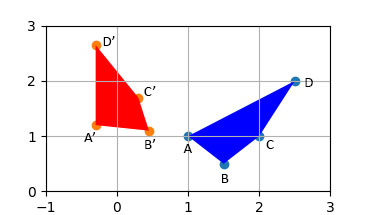
\includegraphics[width=8cm]{quadrilaterals.jpg}

\begin{equation}
\begin{split}
A&=(1, 1)\\
B&=(1.5, 0.5)\\
C&=(2, 1)\\
D&=(2.5, 2)
\end{split}
\quad\quad\quad
\begin{split}
A'&=(-0.3, 1.3)\\
B'&=(0.5, 1.1)\\
C'&=(0.3, 1.8)\\
D'&=(-0.3, 2.6)
\end{split}
\end{equation}

Let's assume that each point in $ABCD$ was approximately mapped to its corresponding point in $A'B'C'D'$ by a $2\times2$ transformation matrix $M$.

e.g. if $A = \begin{pmatrix} x \\ y \end{pmatrix}$ and $A' = \begin{pmatrix} x' \\ y' \end{pmatrix}$, and $\boldsymbol{M} = \begin{pmatrix} m_{1,1} & m_{1,2} \\ m_{2,1} & m_{2,2} \end{pmatrix}$

then $\begin{pmatrix} m_{1,1} & m_{1,2} \\ m_{2,1} & m_{2,2} \end{pmatrix} * \begin{pmatrix} x \\ y \end{pmatrix} \approx \begin{pmatrix} x' \\ y' \end{pmatrix}$

We would like to approximate $\boldsymbol{M}$ using least squares for linear regression.

\begin{enumerate}[(a)]
\item Rewrite the equation $\boldsymbol{M}x \approx x'$ into a pair of linear equations. We have provided you with a template of what they should look like below.

\item Use the equations you wrote for part (a) and coordinate values for $ABCD$ and $A'B'C'D'$ to construct a matrix $\boldsymbol{Q}$ and column vector $b$ that satisfy
\begin{align}
    \boldsymbol{Q}*\begin{pmatrix} m_{1,1} \\ m_{1,2} \\ m_{2,1} \\ m_{2,2} \\ \end{pmatrix} = b
\end{align}

We have provided you with a template of what they should look like below.

\emph{Hint:} You have a pair of equations for each $x$-$x'$ correspondence, giving you $8$ rows in $\boldsymbol{Q}$ and $b$. If you're having trouble, try writing out the equations for each pair of points like in part (a).

\emph{Note:} Systems of linear equations are typically written in the form $\boldsymbol{A}x=b$, but since we have already defined $A$ and $x$, we're writing it as $\boldsymbol{Q}m=b$

\item Our problem is now over-constrained, so we want to find values for $m_{i,j}$ that minimize the squared error between approximated values and real values, or $||\boldsymbol{Q}m-b||_2$. To do this we use singular value decomposition to find the pseudoinverse of $\boldsymbol{Q}$, written as $\boldsymbol{Q}^\dagger$. We then multiply it by both sides, giving us $\boldsymbol{Q}^\dagger \boldsymbol{Q}m = \boldsymbol{Q}^\dagger b \quad\Rightarrow\quad m \approx \boldsymbol{Q}^\dagger b$.

Thankfully, the computer can do all of this for us! \texttt{numpy.linalg.lstsq()} takes in our $\boldsymbol{Q}$ matrix and $b$ vector, and returns approximations for $m$. Plug the values you wrote in part (b) into that function and write the returned $\boldsymbol{M}$ matrix here.
\end{enumerate}

%%%%%%%%%%%%%%%%%%%%%%%%%%%%%%%%%%%
\paragraph{A5:} Your answer here.
% Uncomment the stencil below and fill in your solution.

\begin{enumerate}[(a)]

\item Replace each of the `$\_\_$' below with $x, y, x', y',$ or $0$.
\begin{align}
\begin{cases}
    \_\_m_{1,1} + \_\_m_{1,2} + \_\_m_{2,1} + \_\_m_{2,2} = \_\_ \\
    \_\_m_{1,1} + \_\_m_{1,2} + \_\_m_{2,1} + \_\_m_{2,2} = \_\_
\end{cases}
\end{align}

\item Replace each of the `$\_\_$' below with a $0$ or a coordinate value from $ABCD$ and $A'B'C'D'$.
\begin{align}
    \begin{pmatrix} \_\_ & \_\_ & \_\_ & \_\_ \\ \_\_ & \_\_ & \_\_ & \_\_ \\ \_\_ & \_\_ & \_\_ & \_\_ \\ \_\_ & \_\_ & \_\_ & \_\_ \\ \_\_ & \_\_ & \_\_ & \_\_ \\ \_\_ & \_\_ & \_\_ & \_\_ \\ \_\_ & \_\_ & \_\_ & \_\_ \\ \_\_ & \_\_ & \_\_ & \_\_\end{pmatrix} *\begin{pmatrix} m_{1,1} \\ m_{1,2} \\ m_{2,1} \\ m_{2,2} \\ \end{pmatrix} = \begin{pmatrix} \_\_ \\ \_\_ \\ \_\_ \\ \_\_ \\ \_\_ \\ \_\_ \\ \_\_ \\ \_\_ \end{pmatrix}
\end{align}

\item Replace each of the `$\_\_$' below with the value of $m_{i, j}$.
\begin{align}
    M = \begin{pmatrix} m_{1,1} & m_{1,2} \\ m_{2,1} & m_{2,2} \end{pmatrix} = \begin{pmatrix} \_\_ & \_\_ \\ \_\_ & \_\_ \end{pmatrix}
\end{align}

\end{enumerate}

%%%%%%%%%%%%%%%%%%%%%%%%%%%%%%%%%%%

\pagebreak
\paragraph{Q6:}
In searching for solutions to slow the spread of COVID-19, many governments and organizations have looked to technology, some of which uses cameras and computer vision. Please read these articles on
\href{https://thenextweb.com/neural/2020/03/21/why-ai-might-be-the-most-effective-weapon-we-have-to-fight-covid-19/}{AI usage during the pandemic} and a \href{https://www.bbc.com/news/technology-51439401}{‘close contact detector’}, and answer the following questions.
\begin{enumerate}[(a)]

    \item
    Of the computer vision solutions described, which single solution would you most support and why?
    Which one would you least support and why? (3-4 sentences) \\
    \emph{Note: You may make whichever assumptions you like about how the specific solution might work, but please state them.}

    \item
    Suppose that the `close contact detector' used computer vision as one of its signals, by surreptitiously using your smartphone's cameras along with facial recognition to know who you were near. In a time of crisis, would you be comfortable with this? Why? (3-4 sentences)
\end{enumerate}

The surveillance and biometric measures that help us today may outlast the pandemic and become part of our daily lives.
\begin{enumerate}[(c)]
    \item
    The computer vision technology behind the `close contact detector' starts to be used by governments to locate missing persons and criminal fugitives through your smartphone, without you knowing. Would you be comfortable with this? Why? (3-4 sentences)

    \item
    The technology then becomes commercial software, and it is integrated into a new dating app `Cvpid'. Once installed, as you go about your day, the app passively scans people near you and matches their faces to their social media profiles to find potential partners based on your personal preferences. Would you be comfortable with this? Why? (3-4 sentences)

\end{enumerate}

%%%%%%%%%%%%%%%%%%%%%%%%%%%%%%%%%%%
\paragraph{A6:} Your answer here.
% Uncomment the stencil below and fill in your solution.

% \begin{enumerate}[(a)]

% \item

% \item

% \item

% \item

% \end{enumerate}

%%%%%%%%%%%%%%%%%%%%%%%%%%%%%%%%%%%
% Please leave the pagebreak
\pagebreak
\paragraph{A6 (continued):} Your answer here.

% If you really need extra space, uncomment here and use extra pages after the last question.
% Please refer here in your original answer. Thanks!
%\pagebreak
%\paragraph{AX.X Continued:} Your answer continued here.




%%%%%%%%%%%%%%%%%%%%%%%%%%%%%%%%%%%


%%%%%%%%%%%%%%%%%%%%%%%%%%%%%%%%%%%
\pagebreak
\section*{Feedback? (Optional)}
Please help us make the course better. If you have any feedback for this assignment, we'd love to hear it!


% \pagebreak
% \section*{Any additional pages would go here.}

\end{document}
